%********************************************%
%*       Generated from PreTeXt source      *%
%*       on 2021-03-09T11:36:06+01:00       *%
%*   A recent stable commit (2020-08-09):   *%
%* 98f21740783f166a773df4dc83cab5293ab63a4a *%
%*                                          *%
%*         https://pretextbook.org          *%
%*                                          *%
%********************************************%
%% We elect to always write snapshot output into <job>.dep file
\RequirePackage{snapshot}
\documentclass[oneside,12pt,]{book}
%% Custom Preamble Entries, early (use latex.preamble.early)
%% Default LaTeX packages
%%   1.  always employed (or nearly so) for some purpose, or
%%   2.  a stylewriter may assume their presence
\usepackage{geometry}
%% Some aspects of the preamble are conditional,
%% the LaTeX engine is one such determinant
\usepackage{ifthen}
%% etoolbox has a variety of modern conveniences
\usepackage{etoolbox}
\usepackage{ifxetex,ifluatex}
%% Raster graphics inclusion
\usepackage{graphicx}
%% Color support, xcolor package
%% Always loaded, for: add/delete text, author tools
%% Here, since tcolorbox loads tikz, and tikz loads xcolor
\PassOptionsToPackage{usenames,dvipsnames,svgnames,table}{xcolor}
\usepackage{xcolor}
%% begin: defined colors, via xcolor package, for styling
%% end: defined colors, via xcolor package, for styling
%% Colored boxes, and much more, though mostly styling
%% skins library provides "enhanced" skin, employing tikzpicture
%% boxes may be configured as "breakable" or "unbreakable"
%% "raster" controls grids of boxes, aka side-by-side
\usepackage{tcolorbox}
\tcbuselibrary{skins}
\tcbuselibrary{breakable}
\tcbuselibrary{raster}
%% We load some "stock" tcolorbox styles that we use a lot
%% Placement here is provisional, there will be some color work also
%% First, black on white, no border, transparent, but no assumption about titles
\tcbset{ bwminimalstyle/.style={size=minimal, boxrule=-0.3pt, frame empty,
colback=white, colbacktitle=white, coltitle=black, opacityfill=0.0} }
%% Second, bold title, run-in to text/paragraph/heading
%% Space afterwards will be controlled by environment,
%% independent of constructions of the tcb title
%% Places \blocktitlefont onto many block titles
\tcbset{ runintitlestyle/.style={fonttitle=\blocktitlefont\upshape\bfseries, attach title to upper} }
%% Spacing prior to each exercise, anywhere
\tcbset{ exercisespacingstyle/.style={before skip={1.5ex plus 0.5ex}} }
%% Spacing prior to each block
\tcbset{ blockspacingstyle/.style={before skip={2.0ex plus 0.5ex}} }
%% xparse allows the construction of more robust commands,
%% this is a necessity for isolating styling and behavior
%% The tcolorbox library of the same name loads the base library
\tcbuselibrary{xparse}
%% Hyperref should be here, but likes to be loaded late
%%
%% Inline math delimiters, \(, \), need to be robust
%% 2016-01-31:  latexrelease.sty  supersedes  fixltx2e.sty
%% If  latexrelease.sty  exists, bugfix is in kernel
%% If not, bugfix is in  fixltx2e.sty
%% See:  https://tug.org/TUGboat/tb36-3/tb114ltnews22.pdf
%% and read "Fewer fragile commands" in distribution's  latexchanges.pdf
\IfFileExists{latexrelease.sty}{}{\usepackage{fixltx2e}}
%% Text height identically 9 inches, text width varies on point size
%% See Bringhurst 2.1.1 on measure for recommendations
%% 75 characters per line (count spaces, punctuation) is target
%% which is the upper limit of Bringhurst's recommendations
\geometry{letterpaper,total={408pt,9.0in}}
%% Custom Page Layout Adjustments (use latex.geometry)
\geometry{a4paper,left=3cm,right=3cm,top=2.5cm,bottom=2cm}
%% This LaTeX file may be compiled with pdflatex, xelatex, or lualatex executables
%% LuaTeX is not explicitly supported, but we do accept additions from knowledgeable users
%% The conditional below provides  pdflatex  specific configuration last
%% begin: engine-specific capabilities
\ifthenelse{\boolean{xetex} \or \boolean{luatex}}{%
%% begin: xelatex and lualatex-specific default configuration
\ifxetex\usepackage{xltxtra}\fi
%% realscripts is the only part of xltxtra relevant to lualatex 
\ifluatex\usepackage{realscripts}\fi
%% end:   xelatex and lualatex-specific default configuration
}{
%% begin: pdflatex-specific default configuration
%% We assume a PreTeXt XML source file may have Unicode characters
%% and so we ask LaTeX to parse a UTF-8 encoded file
%% This may work well for accented characters in Western language,
%% but not with Greek, Asian languages, etc.
%% When this is not good enough, switch to the  xelatex  engine
%% where Unicode is better supported (encouraged, even)
\usepackage[utf8]{inputenc}
%% end: pdflatex-specific default configuration
}
%% end:   engine-specific capabilities
%%
%% Fonts.  Conditional on LaTex engine employed.
%% Default Text Font: The Latin Modern fonts are
%% "enhanced versions of the [original TeX] Computer Modern fonts."
%% We use them as the default text font for PreTeXt output.
%% Automatic Font Control
%% Portions of a document, are, or may, be affected by defined commands
%% These are perhaps more flexible when using  xelatex  rather than  pdflatex
%% The following definitions are meant to be re-defined in a style, using \renewcommand
%% They are scoped when employed (in a TeX group), and so should not be defined with an argument
\newcommand{\divisionfont}{\relax}
\newcommand{\blocktitlefont}{\relax}
\newcommand{\contentsfont}{\relax}
\newcommand{\pagefont}{\relax}
\newcommand{\tabularfont}{\relax}
\newcommand{\xreffont}{\relax}
\newcommand{\titlepagefont}{\relax}
%%
\ifthenelse{\boolean{xetex} \or \boolean{luatex}}{%
%% begin: font setup and configuration for use with xelatex
%% Generally, xelatex is necessary for non-Western fonts
%% fontspec package provides extensive control of system fonts,
%% meaning *.otf (OpenType), and apparently *.ttf (TrueType)
%% that live *outside* your TeX/MF tree, and are controlled by your *system*
%% (it is possible that a TeX distribution will place fonts in a system location)
%%
%% The fontspec package is the best vehicle for using different fonts in  xelatex
%% So we load it always, no matter what a publisher or style might want
%%
\usepackage{fontspec}
%%
%% begin: xelatex main font ("font-xelatex-main" template)
%% Latin Modern Roman is the default font for xelatex and so is loaded with a TU encoding
%% *in the format* so we can't touch it, only perhaps adjust it later
%% in one of two ways (then known by NFSS names such as "lmr")
%% (1) via NFSS with font family names such as "lmr" and "lmss"
%% (2) via fontspec with commands like \setmainfont{Latin Modern Roman}
%% The latter requires the font to be known at the system-level by its font name,
%% but will give access to OTF font features through optional arguments
%% https://tex.stackexchange.com/questions/470008/
%% where-and-how-does-fontspec-sty-specify-the-default-font-latin-modern-roman
%% http://tex.stackexchange.com/questions/115321
%% /how-to-optimize-latin-modern-font-with-xelatex
%%
%% end:   xelatex main font ("font-xelatex-main" template)
%% begin: xelatex mono font ("font-xelatex-mono" template)
%% (conditional on non-trivial uses being present in source)
%% end:   xelatex mono font ("font-xelatex-mono" template)
%% begin: xelatex font adjustments ("font-xelatex-style" template)
%% end:   xelatex font adjustments ("font-xelatex-style" template)
%%
%% Extensive support for other languages
\usepackage{polyglossia}
%% Set main/default language based on pretext/@xml:lang value
%% document language code is "es-ES", Spanish
\setmainlanguage{spanish}
%% Enable secondary languages based on discovery of @xml:lang values
%% Enable fonts/scripts based on discovery of @xml:lang values
%% Western languages should be ably covered by Latin Modern Roman
%% end:   font setup and configuration for use with xelatex
}{%
%% begin: font setup and configuration for use with pdflatex
%% begin: pdflatex main font ("font-pdflatex-main" template)
\usepackage{lmodern}
\usepackage[T1]{fontenc}
%% end:   pdflatex main font ("font-pdflatex-main" template)
%% begin: pdflatex mono font ("font-pdflatex-mono" template)
%% (conditional on non-trivial uses being present in source)
%% end:   pdflatex mono font ("font-pdflatex-mono" template)
%% begin: pdflatex font adjustments ("font-pdflatex-style" template)
%% end:   pdflatex font adjustments ("font-pdflatex-style" template)
%% end:   font setup and configuration for use with pdflatex
}
%% Micromanage spacing, etc.  The named "microtype-options"
%% template may be employed to fine-tune package behavior
\usepackage{microtype}
%% Symbols, align environment, commutative diagrams, bracket-matrix
\usepackage{amsmath}
\usepackage{amscd}
\usepackage{amssymb}
%% allow page breaks within display mathematics anywhere
%% level 4 is maximally permissive
%% this is exactly the opposite of AMSmath package philosophy
%% there are per-display, and per-equation options to control this
%% split, aligned, gathered, and alignedat are not affected
\allowdisplaybreaks[4]
%% allow more columns to a matrix
%% can make this even bigger by overriding with  latex.preamble.late  processing option
\setcounter{MaxMatrixCols}{30}
%%
%%
%% Division Titles, and Page Headers/Footers
%% titlesec package, loading "titleps" package cooperatively
%% See code comments about the necessity and purpose of "explicit" option.
%% The "newparttoc" option causes a consistent entry for parts in the ToC 
%% file, but it is only effective if there is a \titleformat for \part.
%% "pagestyles" loads the  titleps  package cooperatively.
\usepackage[explicit, newparttoc, pagestyles]{titlesec}
%% The companion titletoc package for the ToC.
\usepackage{titletoc}
%% Fixes a bug with transition from chapters to appendices in a "book"
%% See generating XSL code for more details about necessity
\newtitlemark{\chaptertitlename}
%% begin: customizations of page styles via the modal "titleps-style" template
%% Designed to use commands from the LaTeX "titleps" package
%% Plain pages should have the same font for page numbers
\renewpagestyle{plain}{%
\setfoot{}{\pagefont\thepage}{}%
}%
%% Single pages as in default LaTeX
\renewpagestyle{headings}{%
\sethead{\pagefont\slshape\MakeUppercase{\ifthechapter{\chaptertitlename\space\thechapter.\space}{}\chaptertitle}}{}{\pagefont\thepage}%
}%
\pagestyle{headings}
%% end: customizations of page styles via the modal "titleps-style" template
%%
%% Create globally-available macros to be provided for style writers
%% These are redefined for each occurence of each division
\newcommand{\divisionnameptx}{\relax}%
\newcommand{\titleptx}{\relax}%
\newcommand{\subtitleptx}{\relax}%
\newcommand{\shortitleptx}{\relax}%
\newcommand{\authorsptx}{\relax}%
\newcommand{\epigraphptx}{\relax}%
%% Create environments for possible occurences of each division
%% Environment for a PTX "chapter" at the level of a LaTeX "chapter"
\NewDocumentEnvironment{chapterptx}{mmmmmm}
{%
\renewcommand{\divisionnameptx}{Capítulo}%
\renewcommand{\titleptx}{#1}%
\renewcommand{\subtitleptx}{#2}%
\renewcommand{\shortitleptx}{#3}%
\renewcommand{\authorsptx}{#4}%
\renewcommand{\epigraphptx}{#5}%
\chapter[{#3}]{#1}%
\label{#6}%
}{}%
%% Environment for a PTX "section" at the level of a LaTeX "section"
\NewDocumentEnvironment{sectionptx}{mmmmmm}
{%
\renewcommand{\divisionnameptx}{Sección}%
\renewcommand{\titleptx}{#1}%
\renewcommand{\subtitleptx}{#2}%
\renewcommand{\shortitleptx}{#3}%
\renewcommand{\authorsptx}{#4}%
\renewcommand{\epigraphptx}{#5}%
\section[{#3}]{#1}%
\label{#6}%
}{}%
%% Environment for a PTX "index" at the level of a LaTeX "chapter"
\NewDocumentEnvironment{indexptx}{mmmmmm}
{%
\renewcommand{\divisionnameptx}{Índice alfabético}%
\renewcommand{\titleptx}{#1}%
\renewcommand{\subtitleptx}{#2}%
\renewcommand{\shortitleptx}{#3}%
\renewcommand{\authorsptx}{#4}%
\renewcommand{\epigraphptx}{#5}%
\chapter*{#1}%
\addcontentsline{toc}{chapter}{#3}
\label{#6}%
}{}%
%%
%% Styles for six traditional LaTeX divisions
\titleformat{\part}[display]
{\divisionfont\Huge\bfseries\centering}{\divisionnameptx\space\thepart}{30pt}{\Huge#1}
[{\Large\centering\authorsptx}]
\usepackage[geometry]{ifsym} %to get nice triangles
\tikzset{weird fill/.style={append after command={
    \pgfextra
        \draw[sharp corners, fill=#1]%
    (\tikzlastnode.west)%
    [rounded corners=0pt] |- (\tikzlastnode.north)%
    [rounded corners=5pt] -| (\tikzlastnode.east)%
    [rounded corners=0pt] |- (\tikzlastnode.south)%
    [rounded corners=5pt] -| (\tikzlastnode.west)%
    ;
    \endpgfextra}}}
\titleformat{name=\chapter}
    {\normalfont}
    {}
    {8pt}
    {
    \begin{center}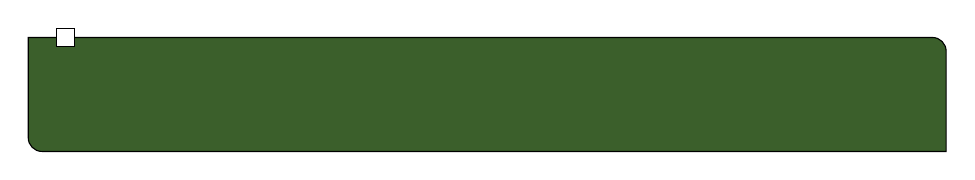
\begin{tikzpicture}
    \draw node[
    inner sep=10pt, inner ysep=20pt, very thick,
    weird fill=colour1, text=white, minimum width={0.9\textwidth},
    text width={0.9\textwidth}, align=center
    ](b) {\scshape\huge\filcenter\titleptx};
    \node[right=10pt, rounded corners=0pt, draw, fill=white] at (b.north west)
    {\divisionnameptx\space\thechapter};
    \end{tikzpicture}\end{center}
    }
    [\hfill{\Large\authorsptx}]
    %%
    \titleformat{name=\chapter,numberless}
    {\normalfont}
    {}
    {8pt}
    {
    \begin{center}\begin{tikzpicture}
    \draw node[
    inner sep=10pt, inner ysep=20pt, very thick,
    weird fill=colour1, text=white, minimum width={0.9\textwidth},
    text width={0.9\textwidth}, align=center
    ](b) {\scshape\huge\filcenter#1};
    \end{tikzpicture}\end{center}
    }
\titleformat{\section}
    {\titlerule
    \vspace{.8ex}%
    \Large\bfseries}
    {\llap{\thesection}}{0.0em}{{\small\FilledSmallTriangleUp}\space\titleptx}
    [\hfill{\large\authorsptx}]
\titleformat{name=\section,numberless}
    {\titlerule
    \vspace{.8ex}%
    \Large\bfseries}
    {}{0.0em}{{\small\FilledSmallTriangleUp}\space#1}
\titleformat{\subsection}{\large\bfseries}
    {\llap{\thesubsection}}{0.0em}{ {\small\FilledSmallTriangleRight\!\!\!\FilledSmallTriangleRight}\space\titleptx}
    [\hfill{\normalsize\authorsptx}]
\titleformat{\subsubsection}{\bfseries}{\llap{\thesubsubsection}}{0.0em}{{\small\FilledSmallTriangleRight\!\!\!\FilledSmallTriangleRight\!\!\!\FilledSmallTriangleRight}\space\titleptx}
    [\hfill{\normalsize\authorsptx}]
\titleformat{\paragraph}[hang]
{\divisionfont\normalsize\bfseries}{\theparagraph}{1em}{#1}
[{\small\authorsptx}]
\titleformat{name=\paragraph,numberless}[block]
{\divisionfont\normalsize\bfseries}{}{0pt}{#1}
[{\normalsize\authorsptx}]
\titlespacing*{\paragraph}{0pt}{3.25ex plus 1ex minus .2ex}{1.5em}
%%
%% Styles for five traditional LaTeX divisions
\titlecontents{part}%
[0pt]{\contentsmargin{0em}\addvspace{1pc}\contentsfont\bfseries}%
{\Large\thecontentslabel\enspace}{\Large}%
{}%
[\addvspace{.5pc}]%
\titlecontents{chapter}%
[0pt]{\contentsmargin{0em}\addvspace{1pc}\contentsfont\bfseries}%
{\large\thecontentslabel\enspace}{\large}%
{\hfill\bfseries\thecontentspage}%
[\addvspace{.5pc}]%
\dottedcontents{section}[3.8em]{\contentsfont}{2.3em}{1pc}%
\dottedcontents{subsection}[6.1em]{\contentsfont}{3.2em}{1pc}%
\dottedcontents{subsubsection}[9.3em]{\contentsfont}{4.3em}{1pc}%
%%
%% Begin: Semantic Macros
%% To preserve meaning in a LaTeX file
%%
%% \mono macro for content of "c", "cd", "tag", etc elements
%% Also used automatically in other constructions
%% Simply an alias for \texttt
%% Always defined, even if there is no need, or if a specific tt font is not loaded
\newcommand{\mono}[1]{\texttt{#1}}
%%
%% Following semantic macros are only defined here if their
%% use is required only in this specific document
%%
%% Used for inline definitions of terms
\newcommand{\terminology}[1]{\textbf{#1}}
%% End: Semantic Macros
%% Division Numbering: Chapters, Sections, Subsections, etc
%% Division numbers may be turned off at some level ("depth")
%% A section *always* has depth 1, contrary to us counting from the document root
%% The latex default is 3.  If a larger number is present here, then
%% removing this command may make some cross-references ambiguous
%% The precursor variable $numbering-maxlevel is checked for consistency in the common XSL file
\setcounter{secnumdepth}{3}
%%
%% AMS "proof" environment is no longer used, but we leave previously
%% implemented \qedhere in place, should the LaTeX be recycled
\newcommand{\qedhere}{\relax}
%%
%% A faux tcolorbox whose only purpose is to provide common numbering
%% facilities for most blocks (possibly not projects, 2D displays)
%% Controlled by  numbering.theorems.level  processing parameter
\newtcolorbox[auto counter, number within=section]{block}{}
%%
%% This document is set to number PROJECT-LIKE on a separate numbering scheme
%% So, a faux tcolorbox whose only purpose is to provide this numbering
%% Controlled by  numbering.projects.level  processing parameter
\newtcolorbox[auto counter, number within=section]{project-distinct}{}
%% A faux tcolorbox whose only purpose is to provide common numbering
%% facilities for 2D displays which are subnumbered as part of a "sidebyside"
\makeatletter
\newtcolorbox[auto counter, number within=tcb@cnt@block, number freestyle={\noexpand\thetcb@cnt@block(\noexpand\alph{\tcbcounter})}]{subdisplay}{}
\makeatother
%%
%% tcolorbox, with styles, for DEFINITION-LIKE
%%
%% definition: fairly simple numbered block/structure
\tcbset{ definitionstyle/.style={
  breakable, colframe=colour2, colback=colour2!5, colbacktitle=colour2!70, coltitle=black, enhanced, attach boxed title to top left={xshift=7mm, yshift*=-2ex},sharp corners=northwest, arc=10pt,
} }
\newtcolorbox[use counter from=block]{definition}[2]{title={{Definición~\thetcbcounter\notblank{#1}{\space\space#1}{}}}, phantomlabel={#2}, breakable, parbox=false, after={\par}, definitionstyle, }
%%
%% tcolorbox, with styles, for EXAMPLE-LIKE
%%
%% example: fairly simple numbered block/structure
\tcbset{ examplestyle/.style={
      enhanced,
      breakable,
      parbox=false,
      frame hidden,
      borderline west={1pt}{0mm}{colour1},
      overlay unbroken and last={
        \draw[colour2, line width=.5pt] (frame.south west) -- (frame.south east);
      },
      colback=white,
      coltitle=white,
      fonttitle=\bfseries\sffamily,
      attach boxed title to top left={xshift=0mm},
      boxed title style={colback=colour1, sharp corners, colframe=colour1},
      boxed title size=title,
      after skip=1em,
      before skip=1em,
    } }
\newtcolorbox[use counter from=block]{example}[2]{title={{Ejemplo~\thetcbcounter\notblank{#1}{\space\space#1}{}}}, phantomlabel={#2}, breakable, parbox=false, after={\par}, examplestyle, }
%%
%% tcolorbox, with styles, for miscellaneous environments
%%
%% assemblage: fairly simple un-numbered block/structure
\tcbset{ assemblagestyle/.style={enhanced, boxrule=0.5pt, sharp corners, colback=colour1!50, colframe=colour1,
colbacktitle=colour1!50, coltitle=black, boxed title style={sharp corners, frame hidden},
fonttitle=\bfseries, attach boxed title to top left={xshift=4mm,yshift=-4mm,yshifttext=-2mm}, top=3mm,
} }
\newtcolorbox{assemblage}[2]{title={\notblank{#1}{#1}{}}, phantomlabel={#2}, breakable, parbox=false, assemblagestyle}
%% Localize LaTeX supplied names (possibly none)
\renewcommand*{\chaptername}{Capítulo}
%% More flexible list management, esp. for references
%% But also for specifying labels (i.e. custom order) on nested lists
\usepackage{enumitem}
%% Support for index creation
%% imakeidx package does not require extra pass (as with makeidx)
%% Title of the "Index" section set via a keyword
%% Language support for the "see" and "see also" phrases
\usepackage{imakeidx}
\makeindex[title=Índice alfabético, intoc=true]
\renewcommand{\seename}{Véase}
\renewcommand{\alsoname}{Véase también}
%% hyperref driver does not need to be specified, it will be detected
%% Footnote marks in tcolorbox have broken linking under
%% hyperref, so it is necessary to turn off all linking
%% It *must* be given as a package option, not with \hypersetup
\usepackage[hyperfootnotes=false]{hyperref}
%% Hyperlinking active in electronic PDFs, all links solid and blue
\hypersetup{colorlinks=true,linkcolor=blue,citecolor=blue,filecolor=blue,urlcolor=blue}
\hypersetup{pdftitle={Matrices y Determinantes}}
%% If you manually remove hyperref, leave in this next command
\providecommand\phantomsection{}
%% Graphics Preamble Entries
\usepackage{tikz}
\usepackage{pgfplots}
\usepackage{pstricks}
\usepackage{phaistos}
\usepackage{xcolor}
%% If tikz has been loaded, replace ampersand with \amp macro
%% extpfeil package for certain extensible arrows,
%% as also provided by MathJax extension of the same name
%% NB: this package loads mtools, which loads calc, which redefines
%%     \setlength, so it can be removed if it seems to be in the 
%%     way and your math does not use:
%%     
%%     \xtwoheadrightarrow, \xtwoheadleftarrow, \xmapsto, \xlongequal, \xtofrom
%%     
%%     we have had to be extra careful with variable thickness
%%     lines in tables, and so also load this package late
\usepackage{extpfeil}
%% Custom Preamble Entries, late (use latex.preamble.late)
%% Begin: Author-provided packages
%% (From  docinfo/latex-preamble/package  elements)
%% End: Author-provided packages
%% Begin: Author-provided macros
%% (From  docinfo/macros  element)
%% Plus three from MBX for XML characters
\newcommand{\order}[1]{\left\lvert#1\right\rvert}
\newcommand{\R}{\mathbb{R}}
\definecolor{colour1}{HTML}{3B5F2B}
\definecolor{colour2}{HTML}{00275F}
\definecolor{colour3}{HTML}{FF8822}
\definecolor{colour4}{HTML}{FF55aa}
\definecolor{azulF}{rgb}{.0,.0,.3}
\newcommand{\lt}{<}
\newcommand{\gt}{>}
\newcommand{\amp}{&}
%% End: Author-provided macros
\begin{document}
\frontmatter
%% begin: half-title
\thispagestyle{empty}
{\titlepagefont\centering
\vspace*{0.28\textheight}
{\Huge Matrices y Determinantes}\\}
\clearpage
%% end:   half-title
%% begin: title page
%% Inspired by Peter Wilson's "titleDB" in "titlepages" CTAN package
\thispagestyle{empty}
{\titlepagefont\centering
\vspace*{0.14\textheight}
%% Target for xref to top-level element is ToC
\addtocontents{toc}{\protect\hypertarget{x:book:matrices}{}}
{\Huge Matrices y Determinantes}\\[3\baselineskip]
{\Large Ricardo Mateos\\
 Cristina Gual\\
 Josu Beobide}\\[0.5\baselineskip]
{\Large Urrutiko Hezkuntzarako Euskal Institutua\\
Instituto Vasco de Eduación a Distancia}\\[3\baselineskip]
{\Large Curso 2020-2021}\\}
\clearpage
%% end:   title page
%% begin: copyright-page
\thispagestyle{empty}
\vspace*{\stretch{2}}
\vspace*{\stretch{1}}
\null\clearpage
%% end:   copyright-page
Teoria y ejercicios de matrices de Matemáticas II.%
%% begin: table of contents
%% Adjust Table of Contents
\setcounter{tocdepth}{1}
\renewcommand*\contentsname{Índice}
\tableofcontents
%% end:   table of contents
\mainmatter
%
%
\typeout{************************************************}
\typeout{Capítulo 1 Matrices}
\typeout{************************************************}
%
\begin{chapterptx}{Matrices}{}{Matrices}{}{}{g:chapter:idp1}
%
%
\typeout{************************************************}
\typeout{Sección 1.1 Definiciones.}
\typeout{************************************************}
%
\begin{sectionptx}{Definiciones.}{}{Definiciones.}{}{}{x:section:sec_definicion_matriz}
\begin{assemblage}{}{g:assemblage:idp2}%
Una \emph{matriz de dimensión \(m \times n\)} es un conjunto de números ordenados en m filas y n columnas de la forma:%
\par
%
\begin{equation*}
A=\begin{pmatrix} 
a_{11} \amp a_{12} \amp \cdots \amp a_{1n} \\
a_{21} \amp a_{22} \amp \cdots \amp a_{2n} \\
\vdots  \amp \vdots  \amp \cdots \amp \vdots \\
a_{m1} \amp a_{m2} \amp \cdots \amp a_{mn} \\
\end{pmatrix}
\end{equation*}
%
\end{assemblage}
Cada elemento genérico de la matriz se designa por \(a_{ij}\), donde \(i\) es el número de fila que ocupa y \(j\) es el número de fila.%
\begin{assemblage}{Igualdad de matrices.}{g:assemblage:idp3}%
Dos matrices de la misma dimensión \(A_{mxn}=(a_{ij})\) y \(B_{mxn}=(b_{ij})\) son iguales si \(a_{ij}=b_{ij}\quad \forall i,j\)%
\end{assemblage}
\begin{example}{}{x:example:ej_matriz1}%
Dada la matriz \(A= \begin{pmatrix}  -1 \amp 1  \\  2 \amp -3 \\  3 \amp -5 \\ \end{pmatrix}\) , escribir su dimensión y los elementos \(a_{12}\), \(a_{22}\) y \(a_{31}\)%
\par\smallskip%
\noindent\textbf{\blocktitlefont Solución}.\hypertarget{g:solution:idp4}{}\quad{}La matriz tiene 3 filas y  2 columnas, luego su dimensión es \(3x2\).%
\par
\(a_{12} = 1\), \(a_{22}= -3\) y \(a_{31}=3\)%
\end{example}
\begin{example}{}{x:example:ej_matriz2}%
Hallar los valores de \(x\) e \(y\) para que las matrices \(\begin{pmatrix}  x \amp 1 \\  2 \amp y \\ \end{pmatrix}\), \(\begin{pmatrix}  3 \amp x-2 \\  y \amp x-1 \\ \end{pmatrix}\) sean iguales.%
\par\smallskip%
\noindent\textbf{\blocktitlefont Solución}.\hypertarget{g:solution:idp5}{}\quad{}Para que sean iguales cada elemento de la primera matriz tiene que ser igual a su correspondiente de la segunda.%
\par
Por lo tanto, \(\begin{cases} x= 3 \cr 1= x-2 \cr 2= y \cr y=x-1 \end{cases}\)%
\par
Resolviendo tenemos que \(x=3 \) e \(y=1\).%
\end{example}
\end{sectionptx}
%
%
\typeout{************************************************}
\typeout{Sección 1.2 Tipos de matrices.}
\typeout{************************************************}
%
\begin{sectionptx}{Tipos de matrices.}{}{Tipos de matrices.}{}{}{x:section:sec_tipos_matrices}
%
\begin{enumerate}[label=\alph*]
\item{}\terminology{Matriz fila}: es la matriz que solo tiene una fila \(A_{1n}\).%
\par
%
\begin{equation*}
A= \begin{pmatrix}  -1 \amp 1  \amp 2  \\ \end{pmatrix}
\end{equation*}
%
\item{}\terminology{Matriz columna}: es la matriz que solo tiene una fila \(A_{m1}\)%
\par
%
\begin{equation*}
A= \begin{pmatrix}  -1 \\  1  \\  2  \\  -3   \\\end{pmatrix}
\end{equation*}
%
\item{}\terminology{Matriz nula}: es la matriz en la que todos sus elementos son nulos.%
\par
%
\begin{equation*}
A= \begin{pmatrix}  0 \amp 0  \\  0  \amp 0 \\   0 \amp 0 \\\end{pmatrix}
\end{equation*}
%
\item{}\terminology{Matriz rectangular}: es la matriz que tiene distinto número de filas que de columnas.%
\par
%
\begin{equation*}
A= \begin{pmatrix}  -1 \amp 1  \amp 2  \\  -3  \amp 3 \amp -5 \\\end{pmatrix}
\end{equation*}
%
\item{}\terminology{Matriz cuadrada}: es la matriz que tiene igual número de filas que de columnas (m=n). En este caso podemos decir que la matriz es de orden n.%
\par
%
\begin{equation*}
B= \begin{pmatrix}  -1 \amp 1  \amp 2  \\  -3  \amp 3 \amp -5 \\  2  \amp 1 \amp 6 \\\end{pmatrix}
\end{equation*}
%
\par
En una matriz cuadrada definimos:%
\par
%
\begin{enumerate}[label=(\roman*)]
\item{}\terminology{Diagonal principal}: Son los elementos cuyo número de fila coincide con el de columna: \(a_{ii}\)%
\par
%
\begin{equation*}
\begin{pmatrix} 
\color{red} 1 \amp -1 \amp 3   \\
0 \amp \color{red}3 \amp 2  \\
3 \amp -2  \amp \color{red}2  \\ 
\end{pmatrix} 
\end{equation*}
%
\item{}\terminology{Diagonal secundaria}: Son todos los elementos tales que \(i+j=n+1\).%
\par
%
\begin{equation*}
\begin{pmatrix} 
1 \amp -1 \amp \color{red} 3   \\
-2 \amp \color{red}{-2} \amp 1   \\
\color{red} 1 \amp -3  \amp -4  \\ 
\end{pmatrix} 
\end{equation*}
%
\end{enumerate}
%
\end{enumerate}
%
\par
Dentro de las matrices cuadradas podemos distinguir las siguientes:%
\par
\terminology{Matrices triangular superior:} Son las que todos sus elementos por debajo de la diagonal principal son cero.%
\par
%
\begin{equation*}
\begin{pmatrix} 
1 \amp -1 \amp 3 \amp 0  \\
\color{red}0 \amp 3  \amp 1 \amp -1  \\
\color{red}0 \amp \color{red}0 \amp 2 \amp 1 \\
\color{red}0 \amp \color{red}0  \amp \color{red}0 \amp -4  \\ 
\end{pmatrix} 
\end{equation*}
%
\par
\terminology{Matrices triangular inferior:} Son las que todos sus elementos por encima de la diagonal principal son cero.%
\par
%
\begin{equation*}
\begin{pmatrix}1 \amp \color{red}0 \amp \color{red}0 \amp \color{red}0  \\
-1 \amp 3  \amp \color{red}0 \amp \color{red}0  \\
1 \amp 2 \amp -2 \amp \color{red}0 \\
4 \amp 0  \amp 6 \amp -2  \\ 
\end{pmatrix} 
\end{equation*}
%
\par
\terminology{Matrices diagonal:} Son las que todos sus elementos fuera de la diagonal principal son cero.%
\par
%
\begin{equation*}
\begin{pmatrix} 1 \amp \color{red}0 \amp \color{red}0 \amp \color{red}0  \\
\color{red}0 \amp 3  \amp \color{red}0 \amp \color{red}0  \\
\color{red}0 \amp \color{red}0 \amp -2 \amp \color{red}0 \\
\color{red}0 \amp \color{red}0  \amp \color{red}0 \amp -2  \\ 
\end{pmatrix}
\end{equation*}
%
\par
\terminology{Matrices escalar:} Son las que todos sus elementos  de la diagonal principal son iguales y el resto cero.%
\par
%
\begin{equation*}
\begin{pmatrix} -2 \amp \color{red}0 \amp \color{red}0 \amp \color{red}0  \\
\color{red}0 \amp -2  \amp \color{red}0 \amp \color{red}0  \\
\color{red}0 \amp \color{red}0 \amp -2 \amp \color{red}0 \\
\color{red}0 \amp \color{red}0  \amp \color{red}0 \amp -2  \\ 
\end{pmatrix}
\end{equation*}
%
\par
\terminology{Matrices identidad:} Son las que todos sus elementos  de la diagonal principal son 1 y el resto cero.%
\par
%
\begin{equation*}
\begin{pmatrix} 1 \amp \color{red}0 \amp \color{red}0 \amp \color{red}0  \\
\color{red}0 \amp 1  \amp \color{red}0 \amp \color{red}0  \\
\color{red}0 \amp \color{red}0 \amp 1 \amp \color{red}0 \\
\color{red}0 \amp \color{red}0  \amp \color{red}0 \amp 1  \\ 
\end{pmatrix}
\end{equation*}
%
\par
La matriz identidad se llama \(I_n\), siendo \(n\) el orden de la matriz.%
\end{sectionptx}
%
%
\typeout{************************************************}
\typeout{Sección 1.3 Operaciones con matrices}
\typeout{************************************************}
%
\begin{sectionptx}{Operaciones con matrices}{}{Operaciones con matrices}{}{}{x:section:sec_operaciones_matrices}
\begin{definition}{Suma.}{g:definition:idp6}%
Dadas dos matrices de la misma dimensión \(A=(a_{ij})\) y \(B=(b_{ij})\) llamamos suma a otra matriz \(C=(c_{ij})\) definida por%
\par
%
\begin{equation*}
(c_{ij})=(a_{ij})+(b_{ij})=(a_{ij}+b_{ij})
\end{equation*}
%
\par
Y cumple las siguientes propiedades%
\par
%
\begin{enumerate}
\item{}\(\displaystyle A+B=B+A\)%
\item{}\(\displaystyle A+(B+C)=(A+B)+C\)%
\item{}\(\displaystyle A+0=A\)%
\item{}\(\displaystyle A-A=0\)%
\end{enumerate}
%
\end{definition}
\begin{example}{}{x:example:exa_oper1}%
Sumar \(\begin{pmatrix}
2 \amp 1 \\
1 \amp 1 \\
3 \amp 2
\end{pmatrix} 
+
\begin{pmatrix}
1 \amp 0 \\
-1 \amp -2 \\
2 \amp 3
\end{pmatrix}    \)%
\par\smallskip%
\noindent\textbf{\blocktitlefont Solución}.\hypertarget{g:solution:idp7}{}\quad{}%
\begin{equation*}
\begin{pmatrix}
2 \amp 1 \\
1 \amp 1 \\
3 \amp 2
\end{pmatrix} 
+
\begin{pmatrix}
1 \amp 0 \\
-1 \amp -2 \\
2 \amp 3
\end{pmatrix}    = 
\begin{pmatrix}
3 \amp 1 \\
0 \amp-1 \\
5 \amp 5
\end{pmatrix}    
\end{equation*}
%
\end{example}
\begin{assemblage}{Producto por un número real.}{g:assemblage:idp8}%
Dados un número real \(k\in \mathbb{R}\) y una matriz \(A=(a_{ij})\) se define el producto de \(k\cdot A\) de la siguiente manera:%
\par
%
\begin{equation*}
k\cdot A=k\cdot (a_{ij})= (k\cdot a_{ij})
\end{equation*}
%
\end{assemblage}
\begin{example}{}{x:example:exa_oper2}%
Realizar la siguiente operación:%
\par
%
\begin{equation*}
5\cdot\begin{pmatrix}
2 \amp 1 \\
1 \amp 1 \\
3 \amp 2
\end{pmatrix}
\end{equation*}
%
\par\smallskip%
\noindent\textbf{\blocktitlefont Solución}.\hypertarget{g:solution:idp9}{}\quad{}%
\begin{equation*}
\begin{pmatrix}
10 \amp 5 \\
5 \amp 5 \\
15 \amp 10
\end{pmatrix}  
\end{equation*}
%
\end{example}
\begin{assemblage}{Producto de matrices.}{g:assemblage:idp10}%
Dos matrices \(A\) y \(B\) se pueden multiplicar si el número de columnas de \(A\) es igual al número de filas de \(B\), en tal caso, se define la multiplicación de la siguiente manera%
\par
%
\begin{equation*}
\underbrace{A}_{m \ast n} \cdot \underbrace{B}_{n\ast p}=\underbrace{C}_{m\ast p}
\end{equation*}
%
\par
Para calcular el elemento \(c_{ij}\) hay que utilizar la fila \(i\) de \(A\) y la columna \(j\) de B.%
\par
%
\begin{equation*}
\begin{pmatrix}
a_{i1} \amp a_{i2}\amp a_{i3}\amp \cdots \amp a_{in} \\
\end{pmatrix}
\cdot
\begin{pmatrix}
a_{j1} \\ a_{j2}\\a_{j3}\\ \cdots \\a_{jn} \\
\end{pmatrix}=a_{i1}\cdot a_{j1}+ a_{i2} \cdot a_{2j} + \cdots +a_{in}\cdot a_{nj}
\end{equation*}
%
\par
\emph{El producto de matrices no es conmutativo \(A \cdot B \neq B\cdot A\)}%
\end{assemblage}
\begin{example}{}{x:example:exa_oper3}%
Realizar el siguiente producto \(\begin{pmatrix}
2 \amp 1 \\
1 \amp 1 \\
3 \amp 2
\end{pmatrix}
\cdot 
\begin{pmatrix}
10 \amp 5 \amp5\\
5 \amp 5 \amp-2
\end{pmatrix}\)%
\par\smallskip%
\noindent\textbf{\blocktitlefont Solución}.\hypertarget{g:solution:idp11}{}\quad{}\(\begin{pmatrix}
2 \amp 1 \\
1 \amp 1 \\
3 \amp 2
\end{pmatrix}
\cdot 
\begin{pmatrix}
10 \amp 5 \amp5\\
5 \amp 5 \amp-2
\end{pmatrix}
=
\begin{pmatrix}
2\cdot 10 + 1 \cdot 5 \amp 2\cdot 5 + 1 \cdot 5 \amp 2\cdot 5 + 1 \cdot (-2)\\
1\cdot 10 + 1 \cdot 5 \amp 1\cdot 5 + 1 \cdot 5 \amp 1\cdot 5 + 1 \cdot (-2)\\
3\cdot 10 + 2 \cdot 5 \amp 3\cdot 5 + 2 \cdot 5 \amp 3\cdot 5 + 2 \cdot (-2)
\end{pmatrix} 
= 
\begin{pmatrix}
25 \amp 15\amp 8)\\
15 \amp 10 \amp 3\\
40 \amp 25 \amp 11
\end{pmatrix}\)%
\end{example}
\begin{example}{}{x:example:exa_oper4}%
Dadas las matrices%
\begin{equation*}
A=\begin{pmatrix}
2\amp2\amp-1 \\
-1\amp-1\amp1 \\
-1\amp-2\amp2
\end{pmatrix}
\qquad
I=\begin{pmatrix}
1\amp0\amp0 \\
0\amp1\amp0 \\
0\amp0\amp1
\end{pmatrix}
\end{equation*}
calcular la matriz \((A-I)^2\)%
\par\smallskip%
\noindent\textbf{\blocktitlefont Solución}.\hypertarget{g:solution:idp12}{}\quad{}%
\par
Primero calculamos \(A-I=\begin{pmatrix}
2\amp2\amp-1 \\
-1\amp-1\amp1 \\
-1\amp-2\amp2
\end{pmatrix}
-
\begin{pmatrix}
1\amp0\amp0 \\
0\amp1\amp0 \\
0\amp0\amp1
\end{pmatrix}
=
\begin{pmatrix}
1 \amp 2 \amp -1 \\
-1\amp-2\amp1 \\
-1\amp-2 \amp 1
\end{pmatrix} \)%
\par
Ahora calculamos \((A-I)^2=\begin{pmatrix}
1 \amp 2 \amp -1 \\
-1\amp-2\amp1 \\
-1\amp-2 \amp 1
\end{pmatrix} 
\cdot
\begin{pmatrix}
1 \amp 2 \amp -1 \\
-1\amp-2\amp1 \\
-1\amp-2 \amp 1
\end{pmatrix} 
=
\begin{pmatrix}
0 \amp 0 \amp 0 \\
0\amp0\amp0 \\
0\amp0 \amp 0
\end{pmatrix} \)%
\end{example}
\begin{example}{}{x:example:exa_oper5}%
Sea \(A=\begin{pmatrix} 1 \amp 0 \\ -1 \amp 1 \end{pmatrix}\). Se pide:%
\par
%
\begin{enumerate}[label=\alph*]
\item{}Demostrar que \(A^2=2A-I\), donde \(I\) es la matriz identidad de orden 2.%
\item{}Expresar \(A^3\) y \(A^4\) en función de \(A\).%
\item{}Calcular \(A^{100}\)%
\end{enumerate}
%
\par\smallskip%
\noindent\textbf{\blocktitlefont Solución}.\hypertarget{g:solution:idp13}{}\quad{}%
\begin{enumerate}[label=\alph*]
\item{}Calculamos \(A^2\)%
\par
\(A^2=\begin{pmatrix} 1 \amp 0 \\ -1 \amp 1 \end{pmatrix} \cdot\begin{pmatrix} 1 \amp 0 \\ -1 \amp 1 \end{pmatrix}= \begin{pmatrix} 1 \amp 0 \\ -2 \amp 1 \end{pmatrix}\)%
\par
Ahora calculamos \(2A-I=2\begin{pmatrix} 1 \amp 0 \\ -1 \amp 1 \end{pmatrix}- \begin{pmatrix} 1 \amp 0 \\ 0 \amp 1 \end{pmatrix}=\begin{pmatrix} 1 \amp 0 \\ -2 \amp 1 \end{pmatrix}\)%
\par
Como vemos son iguales.%
\item{}\(A^3=A^2\cdot A= (2A-I)\cdot A= 2A^2-I\cdot A=2A^2-A=2(2A-I)-A=3A-2I\)%
\par
\(A^4=A^3\cdot A=(3A-2I)\cdot A=3A^2-2I\cdot A= 3(2A-I)-2A=4A-3I\)%
\item{}\(\displaystyle A^{100}=100A-99I=100\begin{pmatrix} 1 \amp 0 \\ -1 \amp 1 \end{pmatrix}- 99\begin{pmatrix} 1 \amp 0 \\ 0 \amp 1 \end{pmatrix}=  \begin{pmatrix} 1 \amp 0 \\ -100 \amp 1 \end{pmatrix}\)%
\end{enumerate}
%
\end{example}
\begin{example}{}{x:example:exa_oper6}%
Dada la matriz \(A=\begin{pmatrix}  0 \amp 0 \amp 1 \\  0 \amp a \amp 0 \\ -1 \amp 0 \amp -2 \end{pmatrix} \), se pide:%
\par
Determínese el valor o los valores del parámetro \(a\) para que se verifique que \(A^2+2A+I=O\), siendo \(I\) la matriz unidad y \(O\) la matriz nula, ambas de orden 3.%
\par\smallskip%
\noindent\textbf{\blocktitlefont Solución}.\hypertarget{g:solution:idp14}{}\quad{}Calculamos \(A^2\)%
\par
%
\begin{equation*}
A^2
=
\begin{pmatrix}
0 \amp 0 \amp 1 \\
0 \amp a \amp 0 \\
-1 \amp 0 \amp -2 
\end{pmatrix}\cdot
\begin{pmatrix}
0 \amp 0 \amp 1 \\
0 \amp a \amp 0 \\
-1 \amp 0 \amp -2 
\end{pmatrix}= 
\begin{pmatrix}
-1 \amp 0 \amp -2 \\
0 \amp a^2 \amp 0 \\
2 \amp 0 \amp 3 
\end{pmatrix}
\end{equation*}
%
\par
Ahora calculamos \(A^2+2A+I\)%
\par
%
\begin{equation*}
\begin{pmatrix}
-1 \amp 0 \amp -2 \\
0 \amp a^2 \amp 0 \\
2 \amp 0 \amp 3 
\end{pmatrix} 
+
2
\begin{pmatrix}
0 \amp 0 \amp 1 \\
0 \amp a \amp 0 \\
-1 \amp 0 \amp -2 
\end{pmatrix}+
\begin{pmatrix}
1 \amp 0 \amp 0 \\
0 \amp 1 \amp 0 \\
0 \amp 0 \amp 1
\end{pmatrix}=
\begin{pmatrix}
0 \amp 0 \amp 0 \\
0 \amp a^2+2a+1 \amp 0 \\
0 \amp 0 \amp 0 
\end{pmatrix}
\end{equation*}
%
\par
Igualando a la matriz nula:%
\par
%
\begin{equation*}
\begin{pmatrix}
0 \amp 0 \amp 0 \\
0 \amp a^2+2a+1 \amp 0 \\
0 \amp 0 \amp 0 
\end{pmatrix}=
\begin{pmatrix}
0 \amp 0 \amp 0 \\
0 \amp 0 \amp 0 \\
0 \amp 0 \amp 0
\end{pmatrix}
\end{equation*}
%
\par
Luego: \(a^2+2a+1=0 \Rightarrow a=-1\)%
\end{example}
\begin{example}{}{x:example:exa_oper7}%
Sean las matrices \(A=\begin{pmatrix} 2 \amp 1 \\ 1 \amp 1 \end{pmatrix}\), \(B=\begin{pmatrix} 1 \amp x \\ x \amp 0  \end{pmatrix}\) y \(C=\begin{pmatrix} 0 \amp -1 \\ -1 \amp 2 \end{pmatrix}\)%
\par
%
\begin{enumerate}[label=\alph*]
\item{}Encuentre el valor o los valores de \(x\) de forma que \(B^2=A\)%
\item{}Determine \(x\) para que \(A+B+C=3I_2\)%
\end{enumerate}
%
\par\smallskip%
\noindent\textbf{\blocktitlefont Solución}.\hypertarget{g:solution:idp15}{}\quad{}%
\begin{enumerate}[label=\alph*]
\item{}Hallamos \(B^2\).%
\par
%
\begin{equation*}
\begin{pmatrix}
1 \amp x \\
x \amp 0 
\end{pmatrix} \cdot 
\begin{pmatrix}
1 \amp x \\
x \amp 0 
\end{pmatrix}=
\begin{pmatrix}
x^2+1 \amp x \\
x \amp x^2
\end{pmatrix}
\end{equation*}
%
\par
Igualamos las dos matrices :%
\par
%
\begin{equation*}
\begin{pmatrix}
x^2+1 \amp x \\
x \amp x^2
\end{pmatrix} =
\begin{pmatrix}
2 \amp 1 \\
1 \amp 1
\end{pmatrix}
\end{equation*}
%
\par
De aquí obtenemos el siguiente sistema de ecuaciones:%
\par
%
\begin{equation*}
\left\lbrace
\begin{array}{l}
x^2+1=2 \\
x=1 \\
x=1 \\
x^2=1
\end{array}
\right. \Rightarrow x=1 
\end{equation*}
%
\item{}Hallamos \(A+B+C\)%
\par
%
\begin{equation*}
\begin{pmatrix}
2 \amp 1 \\
1 \amp 1
\end{pmatrix} +  
\begin{pmatrix}
1 \amp x \\ 
x \amp 0
\end{pmatrix}
+\begin{pmatrix}
0 \amp -1 \\
-1 \amp 2
\end{pmatrix}=
\begin{pmatrix}
3 \amp x \\
x \amp 3
\end{pmatrix}
\end{equation*}
%
\par
Igualando esta matriz a \(3I_2\) obtenemos:%
\par
%
\begin{equation*}
\begin{pmatrix}
3 \amp x \\
x \amp 3
\end{pmatrix}=
\begin{pmatrix}
3 \amp 0 \\
0 \amp 3
\end{pmatrix}
\Rightarrow \left\lbrace
\begin{array}{l}
3=3 \\
x=0 \\
x=0 \\
3=3
\end{array}
\right. \Rightarrow x=0
\end{equation*}
%
\end{enumerate}
%
\end{example}
\end{sectionptx}
\end{chapterptx}
%
\backmatter
%
%
%% A lineskip in table of contents as transition to appendices, backmatter
\addtocontents{toc}{\vspace{\normalbaselineskip}}
%
Las entradas están ordenadas por palabras.%
%
%% The index is here, setup is all in preamble
%% Index locators are cross-references, so same font here
{\xreffont\printindex}
%
\end{document}